\documentclass[17pt,landscape]{foils}
\usepackage[latin1]{inputenc}
\usepackage[T1]{fontenc}
\usepackage[french]{babel}
\usepackage{amsmath,amsthm}
\usepackage{amssymb}
\usepackage{fancyhdr}
\usepackage[pdftex]{graphicx,graphics,color}
\usepackage[colorlinks]{hyperref}
\cfoot{\small{}} \pagestyle{fancy} \hypersetup{pdftitle={A mixed
linear model with change-points for the analysis multiple patients
of CGH data},
           pdfauthor={Emilie LEBARBIER},
           pdfpagemode={FullScreen}
}

\textwidth 24cm \textheight 20cm \topmargin 0cm \oddsidemargin 0cm
\evensidemargin 0cm

\newcommand{\coefbin}[2]{\left(
    \begin{array}{c} #1 \\ #2 \end{array}
  \right)}
  \newcommand{\Bcal}{\mathcal{B}}
\newcommand{\Ccal}{\mathcal{C}}
\newcommand{\Dcal}{\mathcal{D}}
\newcommand{\Ecal}{\mathcal{E}}
\newcommand{\Gcal}{\mathcal{G}}
\newcommand{\Mcal}{\mathcal{M}}
\newcommand{\Ncal}{\mathcal{N}}
\newcommand{\Pcal}{\mathcal{P}}
\newcommand{\Qcal}{\mathcal{Q}}
\newcommand{\Lcal}{\mathcal{L}}
\newcommand{\Tcal}{\mathcal{T}}
\newcommand{\Ucal}{\mathcal{U}}
\newcommand{\alphabf}{\mbox{\mathversion{bold}{$\alpha$}}}
\newcommand{\betabf}{\mbox{\mathversion{bold}{$\beta$}}}
\newcommand{\gammabf}{\mbox{\mathversion{bold}{$\gamma$}}}
\newcommand{\mubf}{\mbox{\mathversion{bold}{$\mu$}}}
\newcommand{\thetabf}{\mbox{\mathversion{bold}{$\theta$}}}
\newcommand{\Pibf}{\mbox{\mathversion{bold}{$\Pi$}}}
\newcommand{\psibf}{\mbox{\mathversion{bold}{$\psi$}}}
\newcommand{\Sigmabf}{\mbox{\mathversion{bold}{$\Sigma$}}}
\newcommand{\taubf}{\mbox{\mathversion{bold}{$\tau$}}}
\newcommand{\Ebf}{{\bf E}}
\newcommand{\Cbf}{{\bf C}}
\newcommand{\Gbf}{{\bf G}}
\newcommand{\Hbf}{{\bf H}}
\newcommand{\Ibf}{{\bf I}}
\newcommand{\mbf}{{\bf m}}
\newcommand{\Obf}{{\bf 0}}
\newcommand{\Rbf}{{\bf R}}
\newcommand{\Sbf}{{\bf S}}
\newcommand{\Tbf}{{\bf T}}
\newcommand{\Ubf}{{\bf U}}
\newcommand{\Vbf}{{\bf V}}
\newcommand{\xbf}{{\bf x}}
\newcommand{\Xbf}{{\bf X}}
\newcommand{\Wbf}{{\bf W}}
\newcommand{\Ybf}{{\bf Y}}
\newcommand{\Zbf}{{\bf Z}}
\newcommand{\Esp}{{\mathbb E}}
\newcommand{\Var}{{\mathbb V}}
\newcommand{\Cov}{{\mathbb C}\mbox{ov}}
\newcommand{\Ibb}{{\mathbb I}}
\newcommand{\Rbb}{\mathbb{R}}
\renewcommand{\baselinestretch}{1.3}
\newdimen\AAdi%
\newbox\AAbo%
\newcommand{\emphase}[1]{\textblue{\sl #1}}
\def\argmax{\mathop{\mathrm{argmax}}}
\newcommand{\ec}[1]{\mathbb{E}_{\phi^{(h)}}\left\{#1 |{\Ybf} \right\}}
\newcommand{\vc}[1]{\mathbb{V}_{\phi^{(h)}}\left\{#1 |{\Ybf} \right\}}
\newcommand{\var}{\mathbb{V}}

\title{\large{A mixed linear model with breakpoints for the
analysis of multiple CGH arrays}}

\author{ E. Lebarbier, S. Robin, B. Thiam \\
      \footnotesize {UMR AgroParisTech/INRA 518, Paris, France} \\
      F. Picard \\
      \footnotesize {UMR CNRS-8071/INRA-1152/Universit\'e d'\'Evry, \'Evry, France}\\
      E. Budinsk\`a \\
      \footnotesize {Institute of Biostatistics and Analyses, Masaryk University, Brno, Czech Republic}  \\ \\ \\
  %\hspace{-3cm}
   { {\sc Workshop Change-Point Detection Methods and Applications}
   11-12/09/08} \\ \\
%Statistics for Systems Biology (SSB) group
   }



\date{}

\begin{document}


\maketitle \MyLogo{}
\definecolor{gris}{rgb}{0.9,0.9,0.9}
\definecolor{bleufonce}{rgb}{0,0,0.5}
%\color{bleufonce} %\pagecolor{gris}
\newcommand{\textblue}[1]{\textcolor{blue}{#1}}
\newcommand{\section}[1]{\centerline{\large \textblue{#1}}}
\newcommand{\paragraph}[1]{\noindent {\textblue{#1}}}
\newcommand{\textred}[1]{\textcolor{red}{#1}}
\newcommand{\textgreen}[1]{\textcolor{green}{ #1}}


%%%%%%%%%%%%%%%%%%%%%%%%%%%%%%%%%%%%%%%%%%%%%%%%%%%%%%%%%%%%%%%%%%%%%%%%%%%%%%%%%%%%%%%%%
%--------------------------------- CGH technology --------------------------------
%%%%%%%%%%%%%%%%%%%%%%%%%%%%%%%%%%%%%%%%%%%%%%%%%%%%%%%%%%%%%%%%%%%%%%%%%%%%%%%%%%%%%%%%
\newpage
\chead{\large {Overview}} \foilhead[-.5in]{}

\begin{enumerate}
\item CGH objective and data. \\

\item Analysis of one CGH profile.
  \begin{itemize}
  \item Segmentation model. \\
  \end{itemize}
\item Analysis of multiple CGH profiles.
\begin{itemize}
\item Mixed linear model with breakpoints.

\item Parameter estimation.
\item Applications. \\
\end{itemize}


\item With large signals? \\

\item Perspectives - Further developments

\end{enumerate}

%%%%%%%%%%%%%%%%%%%%%%%%%%%%%%%%%%%%%%%%%%%%%%%%%%%%%%%%%%%%%%%%%%%%%%%%%%%%%%%%%%%%%%%%%
%--------------------------------- CGH technology --------------------------------
%%%%%%%%%%%%%%%%%%%%%%%%%%%%%%%%%%%%%%%%%%%%%%%%%%%%%%%%%%%%%%%%%%%%%%%%%%%%%%%%%%%%%%%%
\newpage
\chead{\large {CGH microarray technology}} \foilhead[-.5in]{}

%\vspace{-0.3cm}

\paragraph{Objective.} Detection of chromosomal aberrations (within
chromosome). What are the effects of small size DNA
  sequence deletions/amplifications? \\
\centerline{$\rightarrow$ experimental tool: \textblue{microarray
CGH}
  (resolution $\sim$ 100kb)}

\paragraph{CGH = Comparative Genomic Hybridization.} Method for the
  comparative measurement of relative DNA copy numbers between two
  samples (disease/normal, test/reference).


\paragraph{Microarray CGH technology in its principle.}

\vspace{-0.5cm}


\begin{figure}
\begin{center}
\includegraphics[scale=0.47]{principe_CGH.png}
\end{center}
\end{figure}



%\newpage
%\chead{\large {Microarray technology in its principle}}
%\foilhead[-.5in]{}%



%\begin{figure}
%\begin{center}
%\includegraphics{MicroarrayTech.png}
%end{center}
%\end{figure}




%%%%%%%%%%%%%%%%%%%%%%%%%%%%%%%%%%%%%%%%%%%%%%%%%%%%%%%%%%%%%%%%%%%%%%%%%%%%%%%%%%%%%%%%%
%--------------------------------- CGH profile --------------------------------
%%%%%%%%%%%%%%%%%%%%%%%%%%%%%%%%%%%%%%%%%%%%%%%%%%%%%%%%%%%%%%%%%%%%%%%%%%%%%%%%%%%%%%%%
\newpage
\chead{\large {Interpretation of a CGH profile}} \foilhead[-.5in]{}



\begin{figure}
\begin{center}
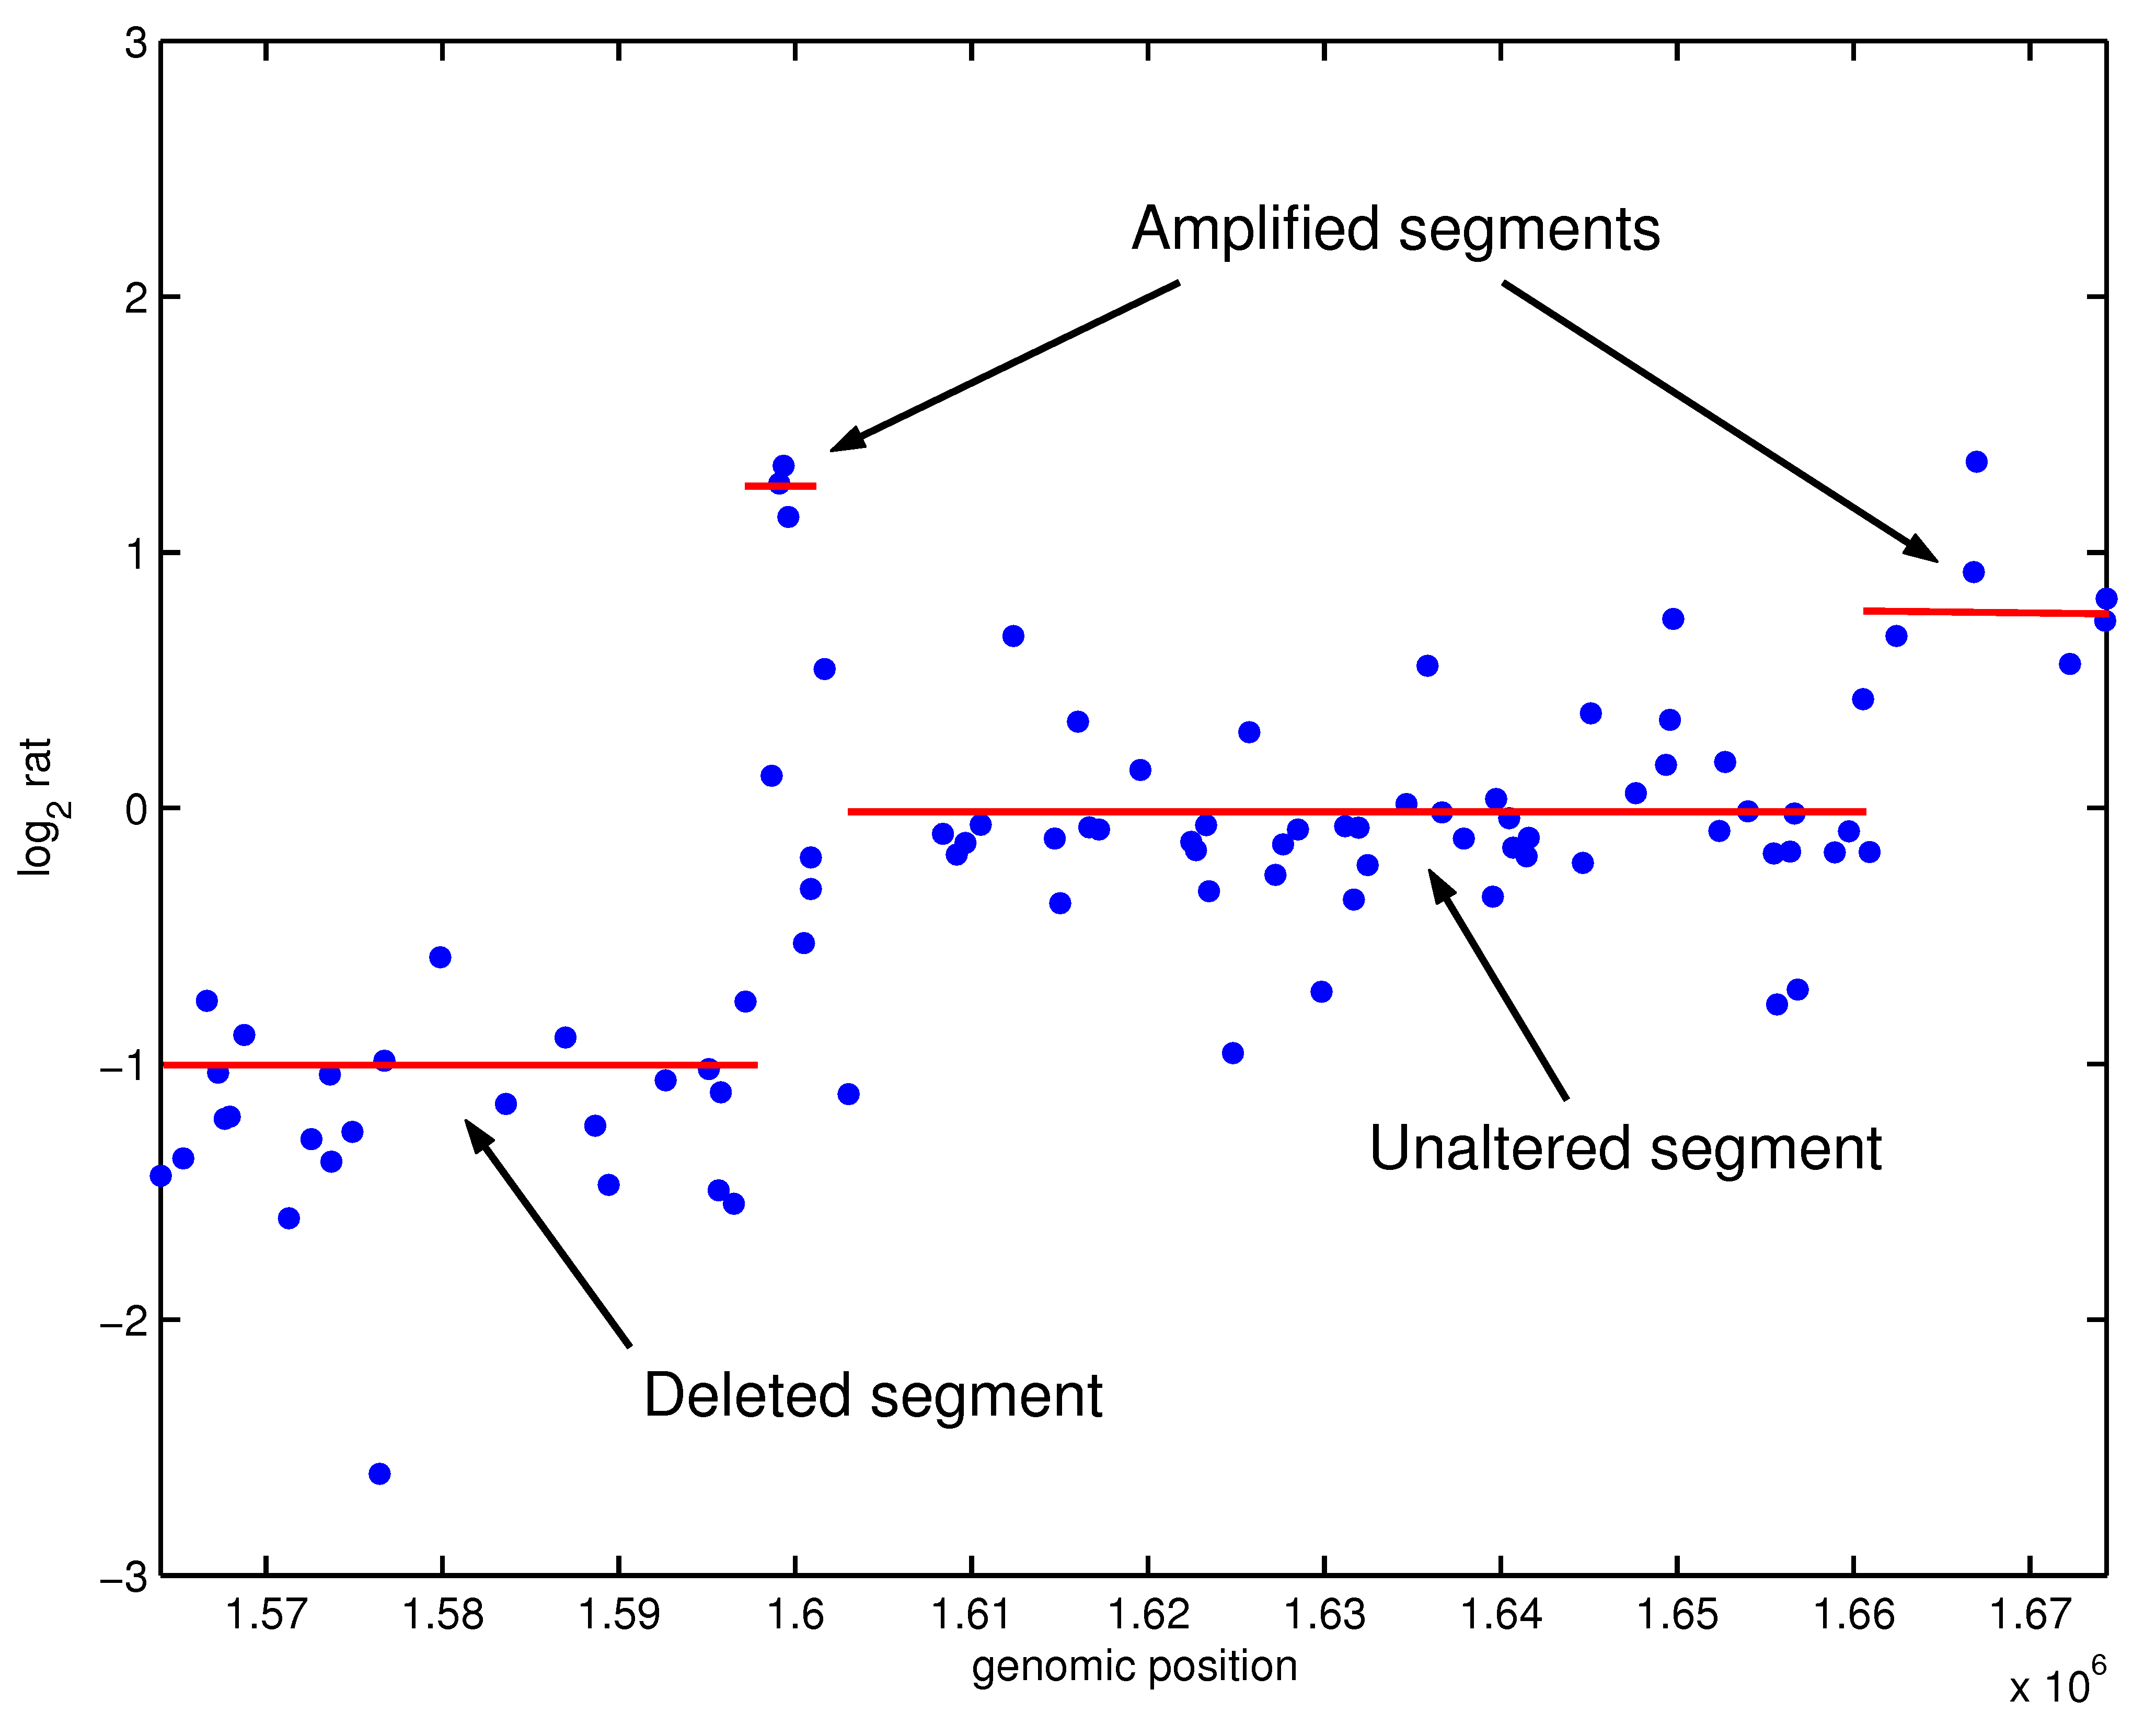
\includegraphics{profile_example.png}
\end{center}
\end{figure}


\centerline{
  A dot on the graph
  $
  \displaystyle{
    = \log_2 \left\{ \frac{\text{ $\sharp$ copies of BAC(t) in the test
          genome }}{\text{$\sharp$ copies of BAC(t) in the reference
          genome}}\right\}}
  $
}


%%%%%%%%%%%%%%%%%%%%%%%%%%%%%%%%%%%%%%%%%%%%%%%%%%%%%%%%%%%%%%%%%%%%%%%%%%%%%%%%%%%%%%%%%
%--------------------------------- Mod�le de d�tection de ruptures --------------------------------
%%%%%%%%%%%%%%%%%%%%%%%%%%%%%%%%%%%%%%%%%%%%%%%%%%%%%%%%%%%%%%%%%%%%%%%%%%%%%%%%%%%%%%%%
\newpage
\chead{\large {Breakpoint detection Model \small{(Work of Picard et
al. (2005))}}} \foilhead[-.5in]{}



\paragraph{Model.} The observed signal $Y=(Y_1,\ldots,Y_n)$ is such that :
$$
Y_t=\mu_k + E_t \ \ \ \  \mbox{ if position $t$ is in segment
$I_k=[t_{k-1}+1,t_{k}]$,}
$$
with $\{E_t\}$ i.i.d. $\sim \Ncal(0,\sigma^2)$ and $k=1,\ldots,K$.

%\vspace{-.2cm}


\paragraph{Parameters.} The parameters of this model are \\
\begin{itemize}

\item the breakpoints
\begin{equation*}
T  =  (t_1, ..., t_{K-1})
\end{equation*}

\item means and variance
\begin{equation*}
\Theta  = (\mu_1,\hdots,\mu_K,\sigma^2)
\end{equation*}
\end{itemize}

%%%%%%%%%%%%%%%%%%%%%%%%%%%%%%%%%%%%%%%%%%%%%%%%%%%%%%%%%%%%%%%%%%%%%%%%%%%%%%%%%%%%%%%%%
%--------------------------------- Mod�le de d�tection de ruptures --------------------------------
%%%%%%%%%%%%%%%%%%%%%%%%%%%%%%%%%%%%%%%%%%%%%%%%%%%%%%%%%%%%%%%%%%%%%%%%%%%%%%%%%%%%%%%%
\newpage
\chead{\large {Estimation of the parameters }} \foilhead[-.5in]{}

\paragraph{Log-Likelihood} (with a constant variance $\sigma^2$):
\begin{eqnarray*}
2 \Lcal_K(T, \Theta) & = & -n \log \sigma^2 - \frac1{\sigma^2}
\sum_{k=1}^K \sum_{t \in
  I_k} (Y_t - \mu_k)^2 + \mbox{cst}.
\end{eqnarray*}


\vspace{-1cm}

\paragraph{When the breakpoints are known.}
$$
\widehat{\mu}_k = \frac1{n_k} \sum_{t \in I_k} Y_t  \ \ , \ \
\widehat{\sigma}^2=\frac1{n} \sum_{k=1}^K \sum_{t \in I_k} (Y_t -
  \widehat{\mu}_k)^2
$$

\vspace{-1cm}
\paragraph{How to find the breakpoints?}


$\rightarrow$ We have to minimize $\sum_{k=1}^K \sum_{t \in I_k}
(Y_t - \widehat{\mu}_k)^2.$

$\rightarrow$ impossible to explore all possible segmentations for
large $n$ and $K$.

$\rightarrow$ Solution: \emphase{dynamic programming} can be used
since the contrast to be minimized is additive in $K$.

\paragraph{Choice of $K$.} Model selection: Penalized
Log-Likelihood.





%%%%%%%%%%%%%%%%%%%%%%%%%%%%%%%%%%%%%%%%%%%%%%%%%%%%%%%%%%
%%%%%%%%%%%%%%%%%%%%%%%%%%%%%%%%%%%%%%%%%%%%%%%%%%%%%%%%%%
\newpage
\chead{\large {Multiple arrays analysis}} \foilhead[-.5in]{}


\paragraph{In the clinical context.} To detect chromosomal aberrations associated with a specific
disease, we compare the profiles of healthy and disease patients, or
the profiles of group of patients with different prognosis.

\paragraph{Aim.} Joint characterization of their CGH profiles.


\paragraph{First approach : common breakpoints:} all patients within the same group have their breakpoints at the
same positions. \\
\noindent $\Rightarrow$ That corresponds to
segment a \textit {multivariate} signal (as many dimensions as
patients): generalization of the model presented above.

%\noindent $\Rightarrow$ Broad diversity of genomic imbalances (even
%for patients with homogeneous diagnosis).


\noindent \textblue{$\Rightarrow$} Common breakpoints: no adapted.

% (broad diversity of genomic imbalances,
%even for patients with homogeneous diagnosis).


%%%%%%%%%%%%%%%%%%%%%%%%%%%%%%%%%%%%%%%%%%%%%%%%%%%%%%%%%%
\newpage
\chead{\large {Correlated profiles}} \foilhead[-.5in]{}



\vspace{1cm}

\hspace{-2cm}
\begin{tabular}{cc}
  \begin{tabular}{p{9cm}}

\paragraph{Proposed model.} \\ \\

$\rightarrow$ We allow patient-specific segmentation. \\ \\

$\rightarrow$ we want to account for \emphase{correlations between
profiles} of patients within a same group at same position.

\\
    \emphase{Probe quality or other technical effect} may alter all the profiles at the same
    position. \\ \\

  \end{tabular}
  &
  \begin{tabular}{l}
    %\begin{figure}
    \includegraphics[scale=0.9]{MixSeg.png}
  %  \end{figure}
  \end{tabular}
\end{tabular}



%%%%%%%%%%%%%%%%%%%%%%%%%%%%%%%%%%%%%%%%%%%%%%%%%%%%%%%%%%
\newpage
\chead{\large {Mixed linear model with breakpoints}}
\foilhead[-.5in]{}


\paragraph{Model.} $Y_{g\ell t}$ denotes the observed logratio at position $t$
for patient $\ell$ within group $g$. We assume that
$$
Y_{g\ell t} = \mu_{g\ell k} + U_{gt} + E_{g\ell t} \qquad \mbox{if
position $t$ belongs to segment $I_{g\ell k}$}
$$
where
\begin{itemize}
\item $I_{g\ell k}$ is the $k$-th segment of patient
  $\ell$ from group $g$,
\item  $\mu_{g\ell k}$ is the mean signal in segment
  $I_{g\ell k}$,
\item  $U_{gt}$ is the random effect at position $t$ in
  group $g$: $\{U_{gt}\}$ independent, $U_{gt} \sim \Ncal(0,
  \sigma^2_g)$,
\item $E_{g\ell t}$ is the noise: $\{E_{g\ell t}\}$
  i.i.d. $\sim \Ncal(0, \sigma^2_0)$.
  \item  $\{E_{g\ell t}\}$ and $\{U_{gt}\}$ independent.   \\
\end{itemize}


$$
\Cov(Y_{g\ell t}, Y_{g'\ell' t'}) =  \sigma^2_g \quad \mbox{ if
  \textblue{same group $g$ and same position $t$}}.
$$


%%%%%%%%%%%%%%%%%%%%%%%%%%%%%%%%%%%%%%%%%%%%%%%%%%%%%%%%%%
\newpage
\chead{\large {General model}} \foilhead[-.5in]{}


$$
\Ybf =  \underset{\mbox{Segmentation}}{\underbrace{\Tbf \mubf}}
+\underset{\mbox{Random effects}}{\underbrace{\Zbf \Ubf}}+
\underset{\mbox{Covariates}}{\underbrace{\Xbf \thetabf}}
 + \Ebf
$$





\begin{eqnarray*}
\left\{   \begin{array}{l} \text{$\mubf$ corresponds to the set of
parameters subject to change,}  \\
\text{$\Tbf$ corresponds to the set of breakpoint positions}
\end{array} \right.
\end{eqnarray*}

\vspace{-1.5cm}


\begin{eqnarray*}
\left\{   \begin{array}{l} \text{$\Ubf$ random effects,}  \\
\text{$\Zbf$ design matrix of the random effects}
\end{array} \right.\\
\end{eqnarray*}

\vspace{-1cm}

\textblue{$\Rightarrow$} Adding covariates in the model :
integration of the experimental design (for example, age of the
patients, sex,... )

\vspace{-2cm}

\begin{eqnarray*}
\left\{   \begin{array}{l} \text{$\thetabf$ constant parameters,}  \\
\text{$\Xbf$ design matrix of the constant parameters}
\end{array} \right.
\end{eqnarray*}


%%%%%%%%%%%%%%%%%%%%%%%%%%%%%%%%%%%%%%%%%%%%%%%%%%%%%%%%%%
\newpage
\chead{\large {General model}} \foilhead[-.5in]{}

where $G = $ number of groups, $L_g =$ number of patients for group
$g$, $n =$ number of positions per profile, $K =$ total number of segments, $N =$ total number of data and \\
\begin{description}
\item[$\bullet \Ubf \; (Gn \times 1)$] \vspace{-0.5cm} (unobserved) and $\sim \Ncal(\Obf, \Gbf)$
  (\emphase{$\Gbf$ diagonal, unknown $\rightarrow$ to estimate}), \\

\item[$\bullet \Ebf \; (N \times 1)$] \vspace{-0.5cm} residual (unobserved):
  $\Ebf \sim \Ncal(\Obf, \Rbf)$ (\emphase{$\Rbf$ diagonal, unknown
    $\rightarrow$ to estimate}), \\

\item[$\bullet \Ubf$ and $\Ebf$] are independent.
\end{description}





%%%%%%%%%%%%%%%%%%%%%%%%%%%%%%%%%%%%%%%%%%%%%%%%%%%%%%%%%%
\newpage
\chead{\large {Estimation of the parameters}} \foilhead[-.5in]{}



\paragraph{Direct maximisation of the likelihood.}
The distribution of $\Ybf$ is
$$
\Ybf \sim \Ncal(\Xbf \thetabf + \Tbf \mubf, \Vbf), \qquad
\mbox{where
  } \Vbf = \Zbf \Gbf \Zbf' + \Rbf.
$$
Because, $\Vbf$ is not diagonal, the direct maximisation of the
observed log-likelihood $\Lcal(\Ybf)$ leads to the minimisation of a
non additive contrast in $K$.

\centerline{Dynamic programming \emphase{can not be used} to
estimate
  $\Tbf$ and $\mubf$}




\paragraph{Conditional distribution.}
$$
\Ybf -\Xbf \thetabf - \Zbf \Ubf \; | \; \Ubf \sim \Ncal(\Tbf \mubf,
\Rbf).
$$
$\Rbf$ is diagonal so the contrast to be minimized is additive in
$K$.

\centerline{\emphase{Dynamic programming can be used to estimate
    $\Tbf$ and $\mubf$}}

\paragraph{Idea.} Mixed models can be viewed as models with incomplete data (\emphase{$U$ is hidden}) whose parameters can be estimated using the E-M
algorithm.





%%%%%%%%%%%%%%%%%%%%%%%%%%%%%%%%%%%%%%%%%%%%%%%%%%%%%%%%%%
\newpage
\chead{\large {E-M algorithm}} \foilhead[-.5in]{}



\paragraph{Principle.} Maximization of the conditional expectation of the complete-data likelihood cond. to $\Ybf$,
$$
\Qcal = \Esp\left[\Lcal(\Ybf, \Ubf; \phi) \; | \; \Ybf \right] =
\underset{\mbox{$\Qcal_0$}}{\underbrace{\Esp\left[\Lcal(\Ybf| \Ubf;
\thetabf,\Tbf,\mubf,\Rbf) \; | \; \Ybf \right]}} +
\underset{\mbox{$\Qcal_1$}}{\underbrace{\Esp\left[\Lcal(\Ubf; \Gbf)
\; | \; \Ybf \right]}}.
$$
where $\phi=(\mubf,\thetabf,\Gbf,\Rbf,\Tbf)$ is the set of
parameters.


 Here we have
\begin{eqnarray*}
  -2\Qcal_0 & = & N\log(2 \pi \sigma^2_0) + \left [ \mbox{\rm Tr}\left[ \Zbf
  \Var(\Ubf|\Ybf) \Zbf'\right] + \|\Ybf - \Xbf\thetabf -
    \Tbf\mubf - \Zbf\Esp(\Ubf|\Ybf) \|^2  \right ] /\sigma^2_0 \\
  \\
  -2\Qcal_1 & = & \sum_g \left[n \log(2\pi\sigma^2_g) +
  \Esp(\Ubf_g'\Ubf_g | \Ybf)/\sigma^2_g \right].
\end{eqnarray*}


%& = & -\frac{1}{2} \left [ M \log(2\pi)+ \log(|\Gbf|)\right ]\\
%              &&-\frac{1}{2} M \text{Tr} \left(\Gbf^{-1}\left[ \ec{\Ubf} \ec{\Ubf}'+\vc{\Ubf} \right] \right)





%%%%%%%%%%%%%%%%%%%%%%%%%%%%%%%%%%%%%%%%%%%%%%%%%%%%%%%%%%
\newpage
\chead{\large {E-M algorithm}} \foilhead[-.5in]{}




\paragraph{E-step.} Calculation of $Q(\phi; \phi^{(h)})=\ec{
    \mathcal{L}(\Ybf,\Ubf;\phi)}$: we need the calculation of \\


the BLUP

\begin{eqnarray*}
  \widehat{\Ubf}^{(h)}&=&\ec{\Ubf}\\
   & = & \Gbf^{(h-1)} \Zbf' \Vbf^{-1} \left (\Ybf-\Xbf
\thetabf^{(h)}-\Tbf ^{(h-1)} \mubf^{(h-1)} \right ),
\end{eqnarray*}
and
\begin{eqnarray*}
\Wbf^{(h)} &=&\vc{\Ubf} \\
& = & \Gbf^{(h-1)} \left [ I_N - \Zbf'
\Vbf^{-1} \Zbf \Gbf^{(h-1)} \right]
\end{eqnarray*}



%%%%%%%%%%%%%%%%%%%%%%%%%%%%%%%%%%%%%%%%%%%%%%%%%%%%%%%%%%
\newpage
\chead{\large {E-M algorithm}} \foilhead[-.5in]{}




\paragraph{M-steps.} Maximization of the obtained $Q(\phi; \phi^{(h)})$. Each step focus on one parameter:

\begin{description}
\item[Estimation of $\thetabf$] with the classical least-squares estimator
\begin{equation*}
  \Xbf' \Rbf^{(h-1)-1} \Xbf \thetabf^{(h)} = \Xbf' \Rbf^{(h-1)-1} (\Ybf
  - \Tbf^{(h-1)} \mubf^{(h-1)}- \Zbf \widehat{\Ubf}^{(h)}).
\end{equation*}

\item[Estimation of the Variances components $\Gbf$ and $\Rbf$,]
(classical maximization)

\item[Estimation of segmentation parameters $\Tbf \mubf$.]

\begin{eqnarray*}
\left\{ \Tbf^{(h)},\mubf^{(h)} \right\} & = & \arg \max_{\Tbf,\mubf}
Q_0 \left(\phi;
  (\thetabf^{(h)},\Gbf^{(h)},\Rbf^{(h)})\right),\\
%&=& \arg\min_{\Tbf\mubf} \|\Ybf - \Xbf
%\thetabf^{(h)}-{\Tbf\mubf}-\Zbf \widehat{\Ubf}^{(h)})\|^2
\end{eqnarray*}
This is equivalent to minimize the residual sum of squares:
\begin{eqnarray*}
RSS_K(\mubf,\Tbf)&=&\|\Ybf - \Xbf \thetabf^{(h)}-{\Tbf\mubf}-\Zbf
\widehat{\Ubf}^{(h)}\|^2
\end{eqnarray*}

\end{description}


%%%%%%%%%%%%%%%%%%%%%%%%%%%%%%%%%%%%%%%%%%%%%%%%%%%%%%%%%%
%%%%%%%%%%%%%%%%%%%%%%%%%%%%%%%%%%%%%%%%%%%%%%%%%%%%%%%%%%
\newpage
\chead{\large {Implementation strategy : the segmentation step}}
\foilhead[-.5in]{}

\paragraph{Optimization problem.} In the case of one group, the purpose is to minimize
\begin{eqnarray*}
RRS_{K}(\mubf, \Tbf) &=&  \sum_{l=1}^{L} \sum_{k=1}^{K_l}
RRS^l_k(\mubf_l,\Tbf_l) =\sum_{l=1}^{L} \sum_{k=1}^{K_l} \sum_{t \in
I_{lk}}\left (\tilde{y}_{lt} -\mu_{lk}\right )^2
\end{eqnarray*}
under the constraint $\sum_l K_l=K$ and with $\tilde{\Ybf}=\Ybf-\Xbf \thetabf^{(h)}-\Zbf \widehat{\Ubf}^{(h)}$. \\


\begin{itemize}
\item This minimization can be achieved thanks to Dynamic
Programming. \\


\item However this is computationally heavy (complexity $\mathcal{O}(n^2 L^2)$).
\end{itemize}



%%%%%%%%%%%%%%%%%%%%%%%%%%%%%%%%%%%%%%%%%%%%%%%%%%%%%%%%%%
%%%%%%%%%%%%%%%%%%%%%%%%%%%%%%%%%%%%%%%%%%%%%%%%%%%%%%%%%%
\newpage
\chead{\large {A new two-stage Dynamic Programming procedure}}
\foilhead[-.5in]{}

\paragraph{We have to}
\begin{equation*}
\min_{\{\Tbf,\mubf\}} RRS_{K}(\mubf, \Tbf)= \min_{K_1+\ldots+K_L=K}
\left \{  \sum_{l=1}^L \min_{\Tbf_l,\mubf_l} RSS^l_{K_l}
(\Tbf_l,\mubf_l) \right \}
\end{equation*}


\paragraph{Proposed strategy.} Two-stage Dynamic Programming
\begin{description}
\item[Stage-1] optimization of $RRS_{K_l}^l$ for each patient $l$ segmented into $K_l$
segments.
\begin{eqnarray*}
\forall l \in [1:L] \ \ \{\hat{\Tbf}_l,\hat{\mubf}_l\}=
\min_{\Tbf_l,\mubf_l} RRS_{K_l}^l.
\end{eqnarray*}


\item[Stage-2] the second step consists in solving:
\begin{eqnarray*}
\min_{K_1+\ldots+K_L=K} \left \{  \sum_{l=1}^L RRS^l_{K_l}
(\hat{\Tbf}_l,\hat{\mubf}_l) \right \}
\end{eqnarray*}
The principle of this stage is to spread $K$ segments among $L$
patients.
\end{description}

\textblue{$\Rightarrow$} This procedure is optimal and with a
complexity $\mathcal{O}( \lambda L n^2 (n+\lambda L^2))$ ($\lambda
<< 1$).






%%%%%%%%%%%%%%%%%%%%%%%%%%%%%%%%%%%%%%%%%%%%%%%%%%%%%%%%%%
\newpage
\chead{\large {Selection of the number of segments $K$}}
\foilhead[-.5in]{}

\paragraph{The total number of breakpoints $K$} is unknown.

\paragraph{Model selection.}
\begin{equation*}
\widehat{K}=\argmax_{K} \left \{ \Lcal(\Ybf; \widehat{\phi})-
\textblue{\alpha}
 \ pen(K) \right \}
\end{equation*}

\paragraph{Penalty.}

\vspace{-1cm}

\begin{eqnarray*}
pen(K)&=& 5 \ \underset{\mbox{Complexity of a model with $K$
segments}} {\underbrace{\text{Number of parameters of a model with
$K$ segments}}} \\
 &&+ 2 \  \underset{\mbox{Number of models with $K$ segments}} {\underbrace{K  \ \log{N/K}}}
\end{eqnarray*}





%$$
%\Ybf =  \underset{\mbox{Segmentation}}{\underbrace{\Tbf \mubf}}
%+\underset{\mbox{Random effects}}{\underbrace{\Zbf \Ubf}}+
%\underset{\mbox{Covariates}}{\underbrace{\Xbf \thetabf}}
% + \Ebf
%$$

\paragraph{Calibration of $\alpha$} by an adaptative method (Birg� and Massart (2004)).





%%%%%%%%%%%%%%%%%%%%%%%%%%%%%%%%%%%%%%%%%%%%%%%%%%%%%%%%%%
%%%%%%%%%%%%%%%%%%%%%%%%%%%%%%%%%%%%%%%%%%%%%%%%%%%%%%%%%%
\newpage
\chead{\large {Application on Nakao dataset - chromosome 20}}
\foilhead[-.5in]{}

\paragraph{Data.} A cohort of $121$ colorectal cancer patients. This
cohort is divided into 4 clinical groups with respective size
$$
L_1=11 \ , \ L_2=37 \ , \ L_3=35 \ \text{and} \ \ L_4=38 \\
$$

\paragraph{Model.}
$$
Y_{g\ell t} = \mu_{g\ell k} + U_{gt} + E_{g\ell t} \qquad \mbox{if
position $t$ belongs to segment $I_{g\ell k}$}
$$
where $\{E_{g\ell t}\} \sim \mathcal{N}(0,\sigma^2_0)$. \\

\paragraph{Variance structure for $\Ubf$.} $\Var(U_{gt})= \sigma^2_g.$






%%%%%%%%%%%%%%%%%%%%%%%%%%%%%%%%%%%%%%%%%%%%%%%%%%%%%%%%%%
\newpage
\chead{\large {Number of breakpoints - $\Var(U_{gt})= \sigma^2_g$ -
$\widehat{K}=240$}} \foilhead[-.5in]{}


\vspace{0.2cm}


\begin{center}
\begin{tabular}{ccc}
  & Stage 1 (11 patients) & Stage 2 (37 patients) \\
  \hspace{-1cm}
  & \begin{tabular}{c}
  \includegraphics[scale=0.45]{hist_ruptures_nakao20_group_Kh=360_group1.png}
  \end{tabular}  &
  \begin{tabular}{c}
  \includegraphics[scale=0.45]{hist_ruptures_nakao20_group_Kh=360_group2.png}
  \end{tabular} \\
 \begin{tabular}{p{5.5cm}} \emphase{Number of breakpoints} \end{tabular} & \\
 \begin{tabular}{p{3.5cm}} \emphase{($\hat{K}$=240)} \end{tabular}&  Stage 3 (35 patients) & Stage 4 (38 patients) \\
  \hspace{-1cm}
 & \begin{tabular}{c}
  \includegraphics[scale=0.45]{hist_ruptures_nakao20_group_Kh=360_group3.png}
  \end{tabular}  &
  \begin{tabular}{c}
  \includegraphics[scale=0.45]{hist_ruptures_nakao20_group_Kh=360_group4.png}
  \end{tabular}
\end{tabular}
\end{center}


%%%%%%%%%%%%%%%%%%%%%%%%%%%%%%%%%%%%%%%%%%%%%%%%%%%%%%%%%%
\newpage
\chead{\large {What is the role of the random effect?}
\emphase{Group 1} ($\widehat{K}_U=240$ and $\widehat{K}_{WU}=230$)}
\foilhead[-.5in]{}

\vspace{-0.5 cm}






\begin{tabular}{c}
  \emphase{\small{Number of patients having a breakpoint at each position with (black) or without (red) random effect}}\\
  \begin{tabular}{c}
  \includegraphics[scale=1.1]{Group1_rupt.png}
  \end{tabular}\\
   \emphase{\small{Predicted random effect} }  \\
  \begin{tabular}{c}
  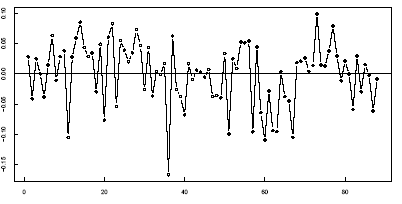
\includegraphics[scale=1.1]{Group1_U.png}
  \end{tabular}
\end{tabular}


%%%%%%%%%%%%%%%%%%%%%%%%%%%%%%%%%%%%%%%%%%%%%%%%%%%%%%%%%%
\newpage
\chead{\large {\emphase{Group 1} : the two profiles with these
changes}} \foilhead[-.5in]{}

\vspace{-.5cm}

\noindent Legend: red$=$without $U$ and black$=$ with $U$.



\begin{figure}
\begin{center}
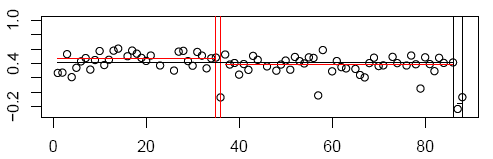
\includegraphics[scale=1]{Exemple_profile6_groupe1.png}
\end{center}
\end{figure}

\begin{figure}
\begin{center}
\includegraphics[scale=1]{Exemple_profile7_groupe1.png}
\end{center}
\end{figure}


%%%%%%%%%%%%%%%%%%%%%%%%%%%%%%%%%%%%%%%%%%%%%%%%%%%%%%%%%%
\newpage
\chead{\large { \emphase{Group 3} (results similar to groups 2 and
4) }} \foilhead[-.5in]{}

\vspace{-0.5 cm}

\begin{tabular}{c}
  \emphase{\small{Number of patients having a breakpoint at each position with (black) or without (red) random effect}}\\
  \begin{tabular}{c}
  \includegraphics[scale=1.1]{Group3_rupt.png}
  \end{tabular}\\
   \emphase{\small{Predicted random effect }}  \\
  \begin{tabular}{c}
  \includegraphics[scale=1.1]{Group3_U.png}
  \end{tabular}
\end{tabular}


%%%%%%%%%%%%%%%%%%%%%%%%%%%%%%%%%%%%%%%%%%%%%%%%%%%%%%%%%%
\newpage
\chead{\large {\emphase{Group 3} : two profiles with these changes}}
\foilhead[-.5in]{}

\vspace{-.5cm}

\noindent Legend: red$=$without $U$ and black$=$ with $U$.




\begin{figure}
\begin{center}
\includegraphics[scale=1]{Exemple_profiles7_24_groupe3_bis.png}
\end{center}
\end{figure}




%%%%%%%%%%%%%%%%%%%%%%%%%%%%%%%%%%%%%%%%%%%%%%%%%%%%%%%%%%
%%%%%%%%%%%%%%%%%%%%%%%%%%%%%%%%%%%%%%%%%%%%%%%%%%%%%%%%%%
\newpage
\chead{\large {Application on Curie dataset (F. Radvanyi)-
chromosome 6}} \foilhead[-.5in]{}

\vspace{-0.5 cm}

\paragraph{Data.} one group of 56 patients with bladder tumors.

\vspace{-0.5 cm}

\begin{tabular}{c}
\emphase{\small{Number of patients having a breakpoint at each position with (+) or without (o) random effect}}  \\
  \begin{tabular}{c}
  \includegraphics[scale=0.7]{histo_rupt_curie.png} \\
  \emphase{\small{Mean segmented profiles (Dotted line: without the random effect. o: with the random effect)}}\\
  \begin{tabular}{c}
  \includegraphics[scale=0.7]{mean_profil_curie.png}
  \end{tabular}\\
  \end{tabular}
\end{tabular}






%%%%%%%%%%%%%%%%%%%%%%%%%%%%%%%%%%%%%%%%%%%%%%%%%%%%%%%%%%
%%%%%%%%%%%%%%%%%%%%%%%%%%%%%%%%%%%%%%%%%%%%%%%%%%%%%%%%%%
\newpage
\chead{\large {Curie dataset - chromosome 6}} \foilhead[-.5in]{}

\begin{tabular}{c}
\emphase{\small{Number of patients having a breakpoint at each position with (+) or without (o) random effect}}  \\
  \begin{tabular}{c}
  \includegraphics[scale=0.7]{histo_rupt_curie.png} \\
  \emphase{\small{Predicted random effect}}\\
  \begin{tabular}{c}
  \includegraphics[scale=0.7]{random_effect_curie.png}
  \end{tabular}\\
  \end{tabular}
\end{tabular}






%%%%%%%%%%%%%%%%%%%%%%%%%%%%%%%%%%%%%%%%%%%%%%%%%%%%%%%%%%
%%%%%%%%%%%%%%%%%%%%%%%%%%%%%%%%%%%%%%%%%%%%%%%%%%%%%%%%%%
\newpage
\chead{\large {3 individual profiles}} \foilhead[-.5in]{}


\hspace{-2cm}
\begin{tabular}{cc}
  \begin{tabular}{p{9cm}}
    The random effect has an influence on the segmentation. \\ \\
    \begin{itemize}
    \item Breakpoints at position 86 are detected in individual
      profiles when analysed independently (\textred{--}).
    \item They vanish after correction of the probe effect vanish
      ({\bf --}).
      \item region at positions 17-19:
amplified region detected for 4/56 patients (gene E2F3 known to be
amplified but not frequently).
    \end{itemize}
  \end{tabular}
  &
  \begin{tabular}{c}
    \includegraphics[scale=0.9]{profils2_9_29.png}
  \end{tabular}
\end{tabular}


%%%%%%%%%%%%%%%%%%%%%%%%%%%%%%%%%%%%%%%%%%%%%%%%%%%%%%%%%%
\newpage
\chead{\large {Interpretation}} \foilhead[-.5in]{}

\begin{itemize}
\item The prediction of the random effect at position 86 is large. \\

\item This position is known to be subject to polymorphism, meaning
that it is altered for many profiles of the cohort.  \\


\item This suggests that the random effect reveals some
particular points, as
\begin{itemize}
\item frequently deleted/amplified position,

\item or points due to technical artefact as for example a bad probe quality or an annotation
error regarding its position in the genome, \\

\end{itemize}

\item whereas the segmentation part of the model $\Tbf \mubf$ reveals
the biological information specific to each profile.

\end{itemize}






%%%%%%%%%%%%%%%%%%%%%%%%%%%%%%%%%%%%%%%%%%%%%%%%%%%%%%%%%%
%%%%%%%%%%%%%%%%%%%%%%%%%%%%%%%%%%%%%%%%%%%%%%%%%%%%%%%%%%
\newpage
\chead{\large {Other application field: harvest dataset (P. Yiou et
al.)}} \foilhead[-.5in]{}

\paragraph{Data.} Harvest dates of 10 cities in France of the years
from 1928 to 2004. \\

\paragraph{Objective.} Detect abrupt
changes in the harvest dates which are not explained by changes in
climate: changes due technical or practical changes.\\

\paragraph{Climatic data.} Mean of the temperatures from April to
August. \\

\paragraph{Model.} $Y_{mt}$ and $x_{mt}$ are the observed harvest date and the temperature at year $t$ for city
$m$:
\begin{equation*}
\forall t \in I_k^{m} \;\; Y_{m t}=\mu_{m k}+b_{m}
x_{mt}+U_{t}+E_{mt}
\end{equation*}
where $\{E_{m t}\} \sim \mathcal{N}(0,\sigma^2_0)$ and $\{U_{t}\}
\sim \mathcal{N}(0,\sigma^2)$.

%%%%%%%%%%%%%%%%%%%%%%%%%%%%%%%%%%%%%%%%%%%%%%%%%%%%%%%%%%
%%%%%%%%%%%%%%%%%%%%%%%%%%%%%%%%%%%%%%%%%%%%%%%%%%%%%%%%%%
\newpage
\chead{\large {Results : $\hat{K}=7$ }} \foilhead[-.5in]{}




\begin{tabular}{c}
\emphase{\small{Number of patients having a breakpoint at each
position}} \\
\emphase{\small{ and Predicted random effect} } \\
  \begin{tabular}{c}
  \includegraphics[scale=1]{U_climat.png} \\
  \end{tabular}
\end{tabular}




%%%%%%%%%%%%%%%%%%%%%%%%%%%%%%%%%%%%%%%%%%%%%%%%%%%%%%%%%%
%%%%%%%%%%%%%%%%%%%%%%%%%%%%%%%%%%%%%%%%%%%%%%%%%%%%%%%%%%
\newpage
\chead{\large {Three profiles }} \foilhead[-.5in]{}




\begin{figure}
\begin{center}
\includegraphics[scale=0.8]{profils_climat1.png}
\end{center}
\end{figure}


The random effect reveals some local (year or period) climatic
effects whereas $b_m$ explains the global relation between the
harvest dates and the climate.




%%%%%%%%%%%%%%%%%%%%%%%%%%%%%%%%%%%%%%%%%%%%%%%%%%%%%%%%%%
%%%%%%%%%%%%%%%%%%%%%%%%%%%%%%%%%%%%%%%%%%%%%%%%%%%%%%%%%%
\newpage
\chead{\large {Segmenting large signals?}} \foilhead[-.5in]{}



\vspace{1cm}

\begin{tabular}{cc}

\begin{tabular}{l}
- With the use of tiling arrays, the size \\
of one signal is huge: $n \sim 10^6$\\ \\
- The complexity of DP is $\mathcal{O}(n^2)$ \\ \\
- DP performs an
exhaustive search, \\
whereas some configurations may not relevant \\ \\
- Reduce the number of configurations \\
 by CART and perform the
exhaustive search on \\
CART-based candidates (Gey $\&$ Lebarbier, 2005).
\end{tabular}

\begin{tabular}{r}
 \includegraphics[scale=0.8]{exemple_CART.png}
\end{tabular}
\end{tabular}



%%%%%%%%%%%%%%%%%%%%%%%%%%%%%%%%%%%%%%%%%%%%%%%%%%%%%%%%%%
%%%%%%%%%%%%%%%%%%%%%%%%%%%%%%%%%%%%%%%%%%%%%%%%%%%%%%%%%%
\newpage
\chead{\large {Perspectives - further developments}}
\foilhead[-.5in]{}


\paragraph{The next step} consists in generalizing the
Segmentation/Clustering framework to the multivariate case (Picard
$\&$ al., 2007).

\paragraph{Objective.} To provide a biological status of the detected
segments: normal/deleted/amplified.

$$
\begin{tabular}{cc}
  \includegraphics[scale=.8]{FigSegClas-1.png} &
  \includegraphics[scale=.8]{FigSegClas-2.png} \\
Segmentation &  Segmentation/Clustering \\
\end{tabular}
$$

%%%%%%%%%%%%%%%%%%%%%%%%%%%%%%%%%%%%%%%%%%%%%%%%%%%%%%%%%%
%%%%%%%%%%%%%%%%%%%%%%%%%%%%%%%%%%%%%%%%%%%%%%%%%%%%%%%%%%
\newpage
\chead{\large {Segmentation/Clustering}} \foilhead[-.5in]{}

\paragraph{General model:}
$$
\Ybf=\Tbf \Cbf \mubf+\Xbf \thetabf+\Zbf \Ubf+\Ebf
$$


\vspace{1cm}
\begin{itemize}
\item $\Cbf$ is the random classification matrix which indicates the
level of each segments, $\Cbf$ is multinomial. \\

\item The estimation procedure is more difficult since $\Ybf | \Ubf,
\Cbf$ is not Gaussian anymore, \\

\item A possibility is to consider the position effect as being
fixed.\\


\item model: for patient $m$
$$
t \in I^m_k, \ k \in p, \ \ \ Y_{mt} \sim \mathcal{N} \left (
\mu_p+\alpha_t,s^2_p\right )
$$
\end{itemize}

%%%%%%%%%%%%%%%%%%%%%%%%%%%%%%%%%%%%%%%%%%%%%%%%%%%%%%%%%%
%%%%%%%%%%%%%%%%%%%%%%%%%%%%%%%%%%%%%%%%%%%%%%%%%%%%%%%%%%
\newpage
\chead{\large {Segmentation/Clustering}} \foilhead[-.5in]{}

\paragraph{Estimation procedure.} An iterative procedure such that

\begin{itemize}
\item Estimation of position effect with the classical least-square
estimator
$$
\alpha^{(h+1)}= \argmax_{\alpha} \log
\mathcal{L}(\Ybf;\Tbf^{(h)},\mubf^{(h)},\alpha)
$$
\item Estimation of the breakpoint positions $\Tbf^{(h+1)}$ with constraint mean
$\mubf^{(h)}$ with
$$
\text{Dynamic Programming}
$$
\item Estimation of the mixture parameters $\mubf^{(h+1)}$ and $\pi^{(h+1)}$ with
$$
\text{E-M algorithm}
$$
\end{itemize}





%%%%%%%%%%%%%%%%%%%%%%%%%%%%%%%%%%%%%%%%%%%%%%%%%%%%%%%%%%
%%%%%%%%%%%%%%%%%%%%%%%%%%%%%%%%%%%%%%%%%%%%%%%%%%%%%%%%%%
\newpage
\chead{\large {Package and documents}} \foilhead[-.5in]{}

\vspace{1cm}

\paragraph{Package.}

We are currently developing an R package to perform all these
multiple sample analysis.

\paragraph{Documents.}

\begin{itemize}

\item Linear Models for multiple segmentation: \textit{Joint segmentation of multivariate Gaussian processes using mixed linear
models.} F. Picard, E. Lebarbier, E. Budinska and S. Robin. \\


\item CART for larger samples: \textit{Using CART to detect multiple change-points in the mean for large
samples.} S. Gey and E. Lebarbier.

\end{itemize}



%%%%%%%%%%%%%%%%%%%%%%%%%%%%%%%%%%%%%%%%%%%%%%%%%%%%%%%%%%
%%%%%%%%%%%%%%%%%%%%%%%%%%%%%%%%%%
% Dernier transparent
\newpage
\chead{\large {}} \foilhead[-.5in]{}


\vspace{5.5cm}

\begin{center}
\Large{Thanks for your attention}
\end{center}



\end{document}
